\documentclass[graybox]{svmult}

\usepackage{booktabs}
\usepackage{cite}
\usepackage[bottom]{footmisc}
\usepackage[utf8]{inputenc}
\usepackage{graphicx}
% epstopdf needs to be included after graphicx.
\usepackage{epstopdf}
\usepackage{listings}
\usepackage{makeidx}
\usepackage{multicol}
\usepackage{newtxtext}
\usepackage{newtxmath}
\usepackage{url}
\RequirePackage[l2tabu, orthodox]{nag}

% Allow PDF 1.7 documents to be included with \includegraphics
\pdfminorversion=7

\graphicspath{{./img/}}

% listing
\lstset{%
  language={C},
  basicstyle={\small\ttfamily},%
  identifierstyle={\small\ttfamily},%
  commentstyle={\small\itshape},%
  keywordstyle={\small\bfseries},%
  ndkeywordstyle={\small\ttfamily},%
  stringstyle={\small\ttfamily},%
  frame={tb},%
  breaklines=true,%
  columns=[l]{fullflexible},%
  numbers=left,%
  numberstyle={\scriptsize},%
  stepnumber=1,%
  numbersep=1em,%
  lineskip=-0.5ex,%
  mathescape,%
  xleftmargin=2em,%
  framexleftmargin=1.5em,%
}

\makeindex

\begin{document}

\title*{An MPI Framework for HPC Clusters Deployed with Software-Defined
Networking}
% Use \titlerunning{Short Title} for an abbreviated version of
% your contribution title if the original one is too long
\author{Keichi Takahashi, Susumu Date, Yasuhiro Watashiba, Yoshiyuki Kido,
Shinji Shimojo}
% Use \authorrunning{Short Title} for an abbreviated version of
% your contribution title if the original one is too long
\institute{Keichi Takahashi \at Nara Institute of Science and Technology,
8916-5 Takayama, Ikoma, Nara, Japan\\ \email{keichi@is.naist.jp}
\and Susumu Date, Yasuhiro Watashiba, Yoshiyuki Kido, Shinji Shimojo \at
Cybermedia Center, Osaka University, 5-1 Mihogaoka, Ibaraki, Osaka, Japan\\
\email{{date, watashiba-y, kido, shimojo}@cmc.osaka-u.ac.jp}}
\maketitle

\abstract*{Lorem ipsum dolor sit amet, consectetuer adipiscing elit. Aenean
commodo ligula eget dolor. Aenean massa. Cum sociis natoque penatibus et
magnis dis parturient montes, nascetur ridiculus mus. Donec quam felis,
ultricies nec, pellentesque eu, pretium quis, sem. Nulla consequat massa quis
enim. Donec pede justo, fringilla vel, aliquet nec, vulputate eget, arcu. In
enim justo, rhoncus ut, imperdiet a, venenatis vitae, justo. Nullam dictum
felis eu pede mollis pretium. Integer tincidunt. Cras dapibus. Vivamus
elementum semper nisi. Aenean vulputate eleifend tellus. Aenean leo ligula,
porttitor eu, consequat vitae, eleifend ac, enim. Aliquam lorem ante, dapibus
in, viverra quis, feugiat a, tellus. Phasellus viverra nulla ut metus varius
laoreet. Quisque rutrum. Aenean imperdiet. Etiam ultricies nisi vel augue.
Curabitur ullamcorper ultricies nisi. Nam eget dui. Lorem ipsum dolor sit
amet, consectetuer adipiscing elit. Aenean commodo ligula eget dolor. Aenean
massa. Cum sociis natoque penatibus et magnis dis parturient montes, nascetur
ridiculus mus. Donec quam felis, ultricies nec, pellentesque eu, pretium quis,
sem. Nulla consequat massa quis enim. Donec pede justo, fringilla vel, aliquet
nec, vulputate eget, arcu. In enim justo, rhoncus ut, imperdiet a, venenatis
vitae, justo. Nullam dictum felis eu pede mollis pretium. Integer tincidunt.
Cras dapibus. Vivamus elementum semper.}


\abstract{Lorem ipsum dolor sit amet, consectetuer adipiscing elit. Aenean
commodo ligula eget dolor. Aenean massa. Cum sociis natoque penatibus et
magnis dis parturient montes, nascetur ridiculus mus. Donec quam felis,
ultricies nec, pellentesque eu, pretium quis, sem. Nulla consequat massa quis
enim. Donec pede justo, fringilla vel, aliquet nec, vulputate eget, arcu. In
enim justo, rhoncus ut, imperdiet a, venenatis vitae, justo. Nullam dictum
felis eu pede mollis pretium. Integer tincidunt. Cras dapibus. Vivamus
elementum semper nisi. Aenean vulputate eleifend tellus. Aenean leo ligula,
porttitor eu, consequat vitae, eleifend ac, enim. Aliquam lorem ante, dapibus
in, viverra quis, feugiat a, tellus. Phasellus viverra nulla ut metus varius
laoreet. Quisque rutrum. Aenean imperdiet. Etiam ultricies nisi vel augue.
Curabitur ullamcorper ultricies nisi. Nam eget dui. Lorem ipsum dolor sit
amet, consectetuer adipiscing elit. Aenean commodo ligula eget dolor. Aenean
massa. Cum sociis natoque penatibus et magnis dis parturient montes, nascetur
ridiculus mus. Donec quam felis, ultricies nec, pellentesque eu, pretium quis,
sem. Nulla consequat massa quis enim. Donec pede justo, fringilla vel, aliquet
nec, vulputate eget, arcu. In enim justo, rhoncus ut, imperdiet a, venenatis
vitae, justo. Nullam dictum felis eu pede mollis pretium. Integer tincidunt.
Cras dapibus. Vivamus elementum semper.}

\section{Introduction}

The demand for computing performance of high-performance computing (HPC)
clusters has been every-growing. In fact, exascale machines are now on the
horizon. To meet the sustained growth of HPC clusters, the high-performance
network that interconnects the compute nodes composing a cluster, or
\textit{interconnect}, needs to be enhanced to achieve larger scale, higher
bandwidth and lower latency. As a result, the interconnect now accounts for a
significant portion of total financial cost and power consumption of an HPC
cluster~\cite{Michelogiannakis2017}.

Until today, the established strategy for designing an interconnect has been
\textit{over-provisioning}, where extra bandwidth and routes are provisioned
in the interconnect. The reason for adopting this design strategy is two-fold.
First, networking hardware used in conventional interconnects do not allow
administrators to change their configurations on-the-fly. Therefore, the
interconnect needs to be provisioned with abundant bandwidth and routes so
that any application with arbitrary communication pattern can experience the
same degree of communication performance. Second, a production HPC cluster is
usually shared among many users where each user runs different applications.
Therefore, tailoring an interconnect to a single application with a specific
communication pattern is unrealistic.


However, an over-subscribed design is becoming increasingly challenging to
implement due to its rapidly rising financial cost and power consumption.
Meanwhile, the assumption that interconnects are static and cannot be
reconfigured does not hold anymore with the recent emergence of networking
technologies that introduces network programmability. A prominent example of
such networking technology is Software-Defined Networking~(SDN), which is a
novel networking architecture that allows administrators to dynamically and
flexibly control the network like a software. We believe that dynamically
controlling the traffic in the interconnect based on the communication pattern
of an application can alleviate traffic congestion in the interconnect and
remove the need for excessive over-provisioning.

Based on this idea, we have been developing on \textit{SDN-enhanced MPI}, a
framework that integrates Software-Defined Networking (SDN) into Message
Passing Interface~(MPI)~\cite{MPIForum2012}. The goal of this framework is to
mitigate congestion in the interconnect and improve MPI communication
performance

dynamically route the traffic in the interconnect based on the communication
patterns of MPI applications with an aim

by utilizing the network programmability provided
by SDN\@. To this end, we have demonstrated that individual MPI collectives
are accelerated by utilizing SDN~\cite{Dashdavaa2014,Takahashi2014}.
Furthermore, we have designed and implemented a mechanism to synchronize the
progress of an application and the reconfiguration of the
interconnect~\cite{Takahashi2015,Takahashi2018}. Furthermore, we have
developed a toolset for facilitating the development of SDN-enhanced MPI that
consists of a profiler to extract communication pattern from applications and
an interconnect simulator to predict the traffic generated in an
interconnect~\cite{Takahashi2017}.

Although our work so far has successfully demonstrated that MPI applications
can be accelerated through the use of of SDN, a key limitation has remained
towards the deployment of our framework on production clusters: our current
SDN-enhanced MPI framework does not support the concurrent execution of
multiple applications on a cluster. As mentioned earlier, clusters are usually
shared among many users. Therefore, it is crucial for the practical use for
our framework that multiple jobs are able to be executed at the same time on a
cluster.

In this paper, we aim to lift this limitation and allow

Specifically, we by integrating our framework
into the job scheduler of a cluster.
The rest of this paper is organized as follows. Section~\ref{kt:sec:ii}
gives an overview of the key technologies behind our proposal and clarifies
the challenges to be tackled. Section~\ref{kt:sec:iii} presents the
architecture of the proposed framework. Section~\ref{kt:sec:iv} shows the
preliminary evaluation result of the proposed framework.
Section~\ref{kt:sec:v} concludes this paper and discusses future work.

\section{Background}\label{kt:sec:ii}

\subsection{Software-Defined Networking (SDN)}

Software-Defined Networking (SDN)~\cite{Jamalian2015} is a novel networking
architecture that brings programmability into the network and allows users to
dynamically and flexibly control the network as if the network was a software.
In conventional networking architectures, the \textit{control plane}, which
makes the decision on how to handle packets, and the \textit {data plane},
which forwards packets, are tightly coupled together on each networking device
such as a switch. In SDN, the two planes are separated into different
hardware. Whereas data plane is implemented on each networking device, the
control plane is handled by a centralized software controller. Administrators
can achieve dynamic and flexible control over the network by developing a
controller that implements their desired control strategy.

The current de facto standard implementation of SDN is
OpenFlow~\cite{McKeown2008}. In an OpenFlow network, the data plane is handled
by OpenFlow switches, whereas the control plane is handled by an OpenFlow
controller. Each OpenFlow switch holds a flow table, which is a collection of
flow entries. A flow entry defines what a matching criteria and action for
incoming packets. The controller is able to control the traffic in the network
by installing and updating the flow table on each switch in the network. This
paper assumes that the interconnect of the cluster is deployed with OpenFlow
switches.

\subsection{Job Scheduler}\label{kt:sec:ii-jms}

A job scheduler is a system that manages the computing resources such as CPU
and memory in a cluster. The job scheduler accepts \textit{job} submissions
from users, which is a request to run an application on the cluster and a set
of resource to run the application. The job scheduler allocates computing
resource in the cluster and launch the application on the allocated computing
resources. If there are not enough available resource in the cluster, the job
will queued for later execution. Job schedulers used in production HPC
clusters include Slurm~\cite{Yoo2003}, PBS
Professional\footnote{\url{https://www.pbspro.org/}},
Torque\footnote{\url{https://www.adaptivecomputing.com/products/torque/}} and
UNIVA Grid Engine\footnote{\url{http://www.univa.com/products/}}. In this
paper, Slurm is assumed since it is one of the most widely adopted open-source
job schedulers.

\begin{figure}
    \centering
    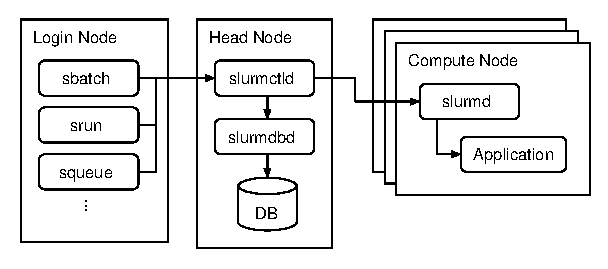
\includegraphics{slurm}
    \caption{Architecture of Slurm}%
    \label{kt:fig:slurm}
\end{figure}

Figure~\ref{kt:fig:slurm} shows the architecture of Slurm. Slurm employs a
\textit{master-worker} architecture like many other job schedulers. The
master, slurmctld, oversees the status of every compute node in the cluster.
It receives job submissions from users, allocates computing resources to a job
and launches the job by instructing to the workers. Optionally, slurmdbd is
used for logging and accounting purposes. Each compute node runs a worker,
slurmd, that monitors the status of the compute, communicates with slurmctld
and launches user applications when requested by slurmctld. Users interact
with slurmctld through utilities such as sbatch (submits a job), srun (submits
an interactive job) and squeue (list queued jobs).

\subsection{Challenges}

As described in Section~\ref{kt:sec:ii-jms}, production HPC clusters usually
employ job schedulers to share their computing resources among multiple
users. Since the job scheduler decides when to run which job, which compute
node to assign to a job, and how to distribute the processes constituting a
job,


Meanwhile, the proposed framework should be transparent from users as much as
possible. A simple approach to obtain node allocation

to run a special daemon within the job. Another. However, both of these
approaches require the user to explicit. Therefore,


\section{Proposal}\label{kt:sec:iii}

This section first briefly reviews the overall architecture of the proposed
framework. Subsequently, individual components of the framework are described
in detail.

\subsection{Overview}



Figure~\ref{kt:fig:architecture} shows the overall architecture of the
proposed SDN-enhanced MPI framework. The proposed framework mainly consists of
three components: (1) interconnect manager, (2) scheduler plugin, and (3)
OpenFlow controller. The interconnect manager is responsible for computing
optimized routes  for each job. The scheduler plugin is responsible
for sending information about a job when a job has started or finished. The
OpenFlow controller is responsible for communicating with the OpenFlow
switches and installing the routing generated by the interconnect manager.
We reuse a generic OpenFlow controller provided by the
Ryu\footnote{\url{https://osrg.github.io/ryu/}} OpenFlow framework that
provides a REST API to install, query, update and remove flows.

\begin{figure}
    \centering
    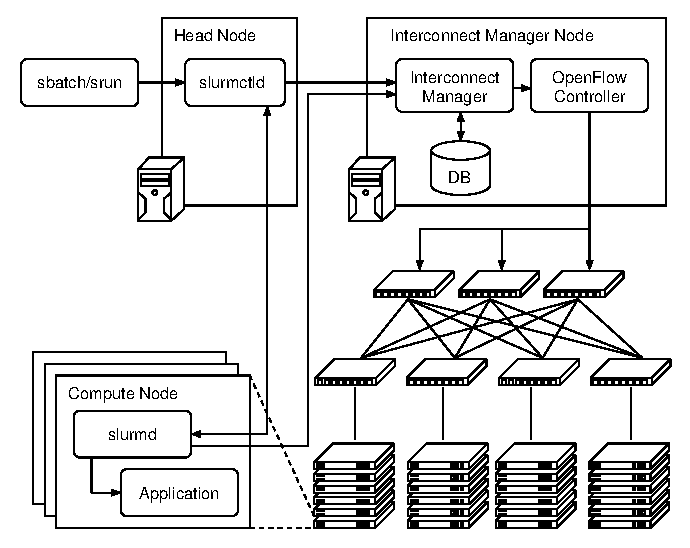
\includegraphics{architecture}
    \caption{Overall architecture}%
    \label{kt:fig:architecture}
\end{figure}

The scheduler plugin and the interconnect manager communicate with
one another using RPCs. Specifically, gRPC\footnote{\url{https://grpc.io/}}, which is an
RPC framework built on top of HTTP/2, is used. The main reason behind this
design choice is because gRPC can automatically generate server and client
codes from an interface definition of remote procedures. Therefore, using gRPC
saves much development effort than implementing our own protocol upon raw
TCP/IP\@.

\subsection{Scheduler Plugin}

The scheduler plugin is responsible for sending information about a job when a
job has started or finished. As described earlier, the scheduler decides when
to run which job. Furthermore, the node allocation and process mapping are
unknown until the job starts. Therefore, a mechanism is needed to notify the
interconnect manager about these information.

For this reason, we utilize a builtin plugin mechanism of Slurm, which is
called Slurm Plug-in Architecture for Node and job Control (SPANK). SPANK
allows developers to easily customize the job startup and cleanup of Slurm.
SPANK plugins are not linked with Slurm itself and can be loaded during
runtime. In addition, SPANK allows developers to add new options to the job
script and job submission commands.

When a job is submitted by a user via sbatch or srun, our plugin sends the ID
and name of the job, uid of the submitter, number of processes and
communication pattern of the application to the interconnect manager. The user
needs to manually specify the communication pattern in the job script as shown
in Listing~\ref{kt:lst:script}.

\begin{lstlisting}[float,caption=An example of a job script,label=kt:lst:script]
#!/bin/bash
#
#SBATCH --job-name=cg-benchmark
#SBATCH --ntasks=128
#SBATCH --time=01:00:00
#
#SBATCH --comm-pattern=cg-c-128
\end{lstlisting}

When a job is being launched on each compute node by slurmd, our plugin sends
the ID and name of the job, node ID and MPI rank number to the interconnect
manager. These information is used by the interconnect manager to obtain the
node allocation and process mapping. After these information are sent over to
the interconnect manager, the plugin blocks until the routings are computed
and installed to the interconnect. Once the routings are ready, the plugin
returns control to Slurm and eventually, the user application is started.

When a job has finished, the same information is send over to the interconnect
manager. Similar to the launch, the plugin blocks until the routings are
uninstalled from the interconnect. After that, the rest of the cleanup is
resumed.

All of the above operations are performed transparently from the user
application. In other words, the user application does not need to be modified
nor a special program needs to be executed in the job.

\subsection{Interconnect Manager}

The primary purpose of the interconnect manager is to compute and install
optimal routing for each job.

To compute the optimal routing, the interconnect manager needs to know how
the MPI processes constituting a job is laid out in the cluster. These
information are received from the scheduler plugin integrated into the Slurm
scheduler. Furthermore, the communication pattern of a job is also received
from the plugin if the user has specified the communication pattern. These
information are kept on an external database (currently
SQLite\footnote{\url{https://www.sqlite.org/index.html}} is used) for
fault-tolerance and having multiple instances of the interconnect manager.

Once received these information from the scheduler plugin, the interconnect
manager computes the optimal routing for based on these information.
The routing algorithm is pluggable and can be swapped out. The computed
routing is then installed through the OpenFlow controller to each switch in
the interconnect.

\section{Evaluation}\label{kt:sec:iv}

In this section, we conduct a preliminary evaluation to assess the
effectiveness of our proposed framework.

\subsection{Evaluation Environment}

The evaluation experiment was conducted on a small-scale cluster composed of
20 compute nodes connected through a two-tier fat-tree interconnect as
illustrated in Fig.~\ref{kt:fig:cluster}. Each compute node is equipped with
two quad-core Intel Xeon E5520 CPUs, resulting in a total of 160 cores in the
cluster. A single NEC PF5240 OpenFlow switch is divided into six virtual
switches to compose a fat-tree topology. D-mod-K routing~\cite{Rodriguez2009}
was chosen as the representative example of a conventional routing. D-mod-K
routing statically distributes the routes across multiple paths in the
interconnect.

\begin{figure}
    \centering
    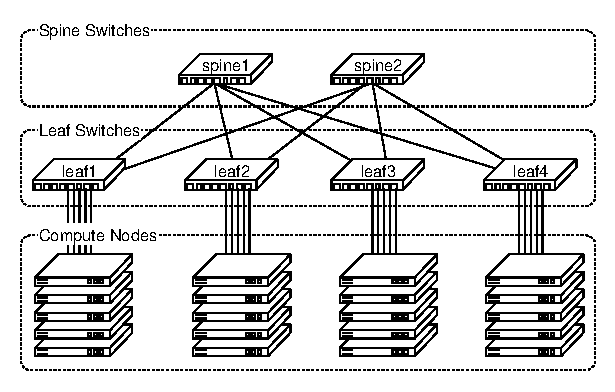
\includegraphics{evaluation_cluster}
    \caption{Cluster used for evaluation}%
    \label{kt:fig:cluster}
\end{figure}

We executed a set of benchmarks on a cluster and compared the communication
time of each benchmark with and without our framework.
Table~\ref{kt:tbl:miniapps} shows a list of communication benchmarks used in
the evaluation. CG and FT are taken from the NAS parallel benchmark
suite~\cite{Bailey1991}. Stencil2D, Stencil3D and SpMV are developed by us.
All benchmarks were executed with 160 processes. In other words, we ran a
single process for every CPU core in the cluster.

\begin{table}
\caption{Benchmarks used in the evaluation}%
\label{kt:tbl:miniapps}
\begin{tabular}{ll}
\toprule
Name      & Description \\ \midrule
CG        & Solves a sparse linear system using the conjugate gradient method \\
FT        & Solves partial differential equation using FFT and IFFT           \\
Stencil2D & A two-dimensional stencil code                                    \\
Stencil3D & A three-dimensional stencil code                                  \\
Butterfly & A three-dimensional stencil code                                  \\
SpMV      & A sparse matrix-vector multiplication kernel                      \\ \bottomrule
\end{tabular}
\end{table}

\subsection{Evaluation Result}

Figure~\ref{kt:fig:benchmark} shows the relative speedup of communication time
when using our framework compared to D-mod-K routing. CG, Butterfly, and SpMV
achieved 1.29$\times$, 1.18$\times$, and 2.56$\times$ speedup, respectively.
In contrast, FT, Stencil2D, and Stencil3D did not exhibit a clear performance
gain by using our framework.

We believe this trend can be explained from the following reason. FT performs
all-to-all communication between processes. This lack of locality makes it
challenging to efficiently map the communication pattern into the interconnect
In contrast, Stencil2D and Stencil3D perform nearest neighbor communication in
a two-dimensional or three-dimensional process grid. As a result, most of the
communication happens within a compute node or within a leaf switch, which
makes the difference in routing algorithms irrelevant.

The three benchmarks that benefited from our framework (CG, Butterfly and
SpMV) perform both local and remote communication between processes.
Therefore, it is possible to efficiently utilize the multiple paths in the
interconnect.

\begin{figure}
    \centering
    \includegraphics{benchmark_result}
    \caption{Benchmark results using miniapps}%
    \label{kt:fig:benchmark}
\end{figure}

\section{Conclusion}\label{kt:sec:v}

In this paper,

As a future work,

\begin{acknowledgement}
This work was supported by JSPS KAKENHI Grant Number 17K00168.
\end{acknowledgement}

\bibliographystyle{spmpsci}
\bibliography{references}

\end{document}
